\documentclass{snedecorbeamer}

%% Diagrams
\usepackage{tikz}
\usetikzlibrary{positioning,decorations.pathreplacing,quotes,overlay-beamer-styles}

%% https://tex.stackexchange.com/a/117661
\AtBeginSection{\frame{\sectionpage}}
\AtBeginSubsection{\frame{\subsectionpage}}

% Setup ------------------------------------------------------------------------
\graphicspath{{include/}}

\title{\textbf{Automatic Relevance Determination} \\
  for Gaussian Processes with Functional Inputs}

\renewcommand*{\thefootnote}{\fnsymbol{footnote}}
\author[Damiano et al]{
  \textbf{Luis Damiano}\footnote[2]{
    \tiny{\href{mailto:ldamiano@iastate.edu}{ldamiano@iastate.edu}}
  }}

\institute{
  Department of Statistics, Iowa State University
}

\date[December 19th, 2022]{
  \tiny{Argonne National Laboratory \\
    MCS Mathematics and Computer Science} \\
  December 19th, 2022}

\begin{document}

% Title page -------------------------------------------------------------------
\begin{frame}
  \titlepage{}
  {
    \tiny{
      Funded, in part, by
      \begin{itemize}
      \item[-] ISU Presidential Interdisciplinary
	Research Initiative on C-CHANGE:~Science for a Changing
	Agriculture
      \item[-] Foundation for Food and Agriculture Research
	Grant ID: CA18-SS-0000000278
      \end{itemize}
    }
  }
\end{frame}

% Introduction -----------------------------------------------------------------
%
\section{Motivation}

\begin{frame}
  \frametitle{Automatic Relevance Determination}
  \framesubtitle{What is it?}

  Text
\end{frame}

\begin{frame}
  \frametitle{Functional input computer experiments}
  \framesubtitle{What is it?}

  \begin{table}[]
    \footnotesize
    \begin{tabular}{@{}lllll@{}}
      \toprule
      \small Output
      & \begin{tabular}[c]{@{}l@{}}\small Input\\ $X(t): \mathcal{T} \to
	  \mathbb{R}$\end{tabular}
      & \begin{tabular}[c]{@{}l@{}}\small Index\\ $t \in \mathcal{T}$\end{tabular}
      & \begin{tabular}[c]{@{}l@{}}\small Index subspaces\\ $t \in
	  \mathcal{T}_u$\end{tabular}
      & \small Mechanism \\ \midrule
      Plant growth
      & Phosphorus
      & Depth
      & Soil layers
      & Root biomass \vspace{1ex}
      \\
      & Precipitation
      & Time
      & Cycles, seasons
      &
	\begin{tabular}[c]{@{}l@{}}
	  Germination \\photosynthesis \\ nutrient absorption
	\end{tabular}
      \vspace{1ex}
      \\
      Soil erosion
      & Elevation
      & Distance
      & Up/down slope
      & Water erosion \vspace{1ex}
      \\
      Radiance
      & Chemical species
      & Elevation
      & Atmospheric layers
      & Reflectivity \vspace{0ex}
      \\
      \bottomrule
    \end{tabular}
  \end{table}

  \vfill
  \begin{quote}
    Index subspaces can provide a meaningful representation of the
    physical process
  \end{quote}

  \vfill
  \begin{quote}
    Can we establish an explicit link $X(t) \xrightarrow{f} y$ for UQ?%
  \end{quote}
\end{frame}

\begin{frame}[c]
  \frametitle{ARD + Functional inputs}
  \framesubtitle{What is the state of the art?}

  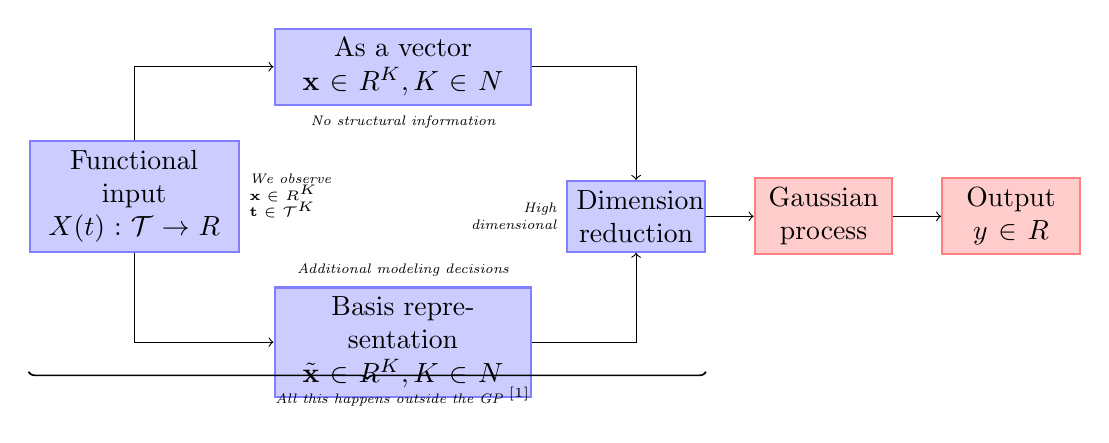
\begin{tikzpicture}
  [
  txtbox1/.style={rectangle,align=center,draw=blue!50,fill=blue!20,thick},
  txtbox2/.style={rectangle,align=center,draw=red!50,fill=red!20,thick},
  every label/.style={font=\itshape\tiny}
  ]

  \node (inp)  [txtbox1] at ( 0,  0) [text width=16ex]
  [label={[align=left]right:We observe \\ $\mathbf{x} \in \mathbb{R}^K$\\ $\mathbf{t}\in\mathcal{T}^K$}] {
    Functional input \\
    $X(t): \mathcal{T} \to \mathbb{R}$
  };
  \node (vec1) [txtbox1] [above right=4ex of inp]   [text width=20ex]
  [label=below:No structural information]{
    As a vector \\
    $\mathbf{x} \in \mathbb{R}^K, K \in \mathbb{N}$
  };
  \node (vec2) [txtbox1] [below right=4ex of inp]   [text width=20ex]
  [label=above:Additional modeling decisions]{
    Basis representation \\
    $\tilde{\mathbf{x}} \in \mathbb{R}^K, K \in \mathbb{N}$
  };

  \node (dred) [txtbox1] [above right=4ex of vec2] [text width=10ex]
  [label={[align=right]left:High\\dimensional}]
  {
    Dimension \\ reduction
  };

  \node (gp)   [txtbox2] [right=4ex of dred] [text width=10ex] {
    Gaussian \\ process
  };
  \node (out)  [txtbox2] [right=4ex of gp] [text width=10ex]  {
    Output \\ $y \in \mathbb{R}$
  };

  \node [below=6ex of vec2.north, label=below:All this happens outside the GP$~^{[1]}$] {
  };

  \draw [->] (inp.north) |- (vec1.west);
  \draw [->] (inp.south) |- (vec2.west);
  \draw [->] (vec1.east) -| (dred.north);
  \draw [->] (vec2.east) -| (dred.south);
  \draw [->] (dred.east) -- (gp.west);
  \draw [->] (gp.east)   -- (out.west);
  \path (inp.south west)
  edge[decorate,decoration={brace,mirror,raise=10ex},line width=.6pt]
  (inp.south west -| dred.south east);
\end{tikzpicture}

%%% Local Variables:
%%% mode: latex
%%% TeX-master: t
%%% End:


  \blankfootnote{
    $~^{[1]}$\cite{muehlenstaedt2017,nanty2016,wang2017,tan2019,wang2019,betancourt2020,betancourt2020a,li2021} \,
    $~^{[2]}$\cite{morris2012,kuttubekova2019}
    Add a keyword (e.g., PCA, FPCA, etc)
  }
\end{frame}

% Automatic Dynamic Relevance Determination ------------------------------------
\section{Automatic \textit{Dynamic} Relevance Determination}

\begin{frame}
  \frametitle{Automatic Dynamic Relevance Determination}
  \framesubtitle{Framework}

  A bunch of slides here
\end{frame}

% Microwave Limb Sounder -------------------------------------------------------
\section{NASA's Microwave Limb Sounder \\ {\small a case study}}

\begin{frame}
  \frametitle{The science}
  \framesubtitle{Explain the science here}

  A satellite image (left)

  An example of the profiles but with the atmospheric rule
\end{frame}

\begin{frame}
  \frametitle{Methods}
  \framesubtitle{Model}

  Introduce the ALF

  Equation, but also the curves
\end{frame}

\begin{frame}
  \frametitle{Methods}
  \framesubtitle{Implementation}

  Implementation details
\end{frame}

\begin{frame}
  \frametitle{Results}
  \framesubtitle{Posterior for model interpretation}

  Figure with posterior weights for fiGP
\end{frame}

\begin{frame}
  \frametitle{Results}
  \framesubtitle{Posterior for model comparison}

  Figure with posterior weights for fiGP vs viGP
\end{frame}

\begin{frame}
  \frametitle{Results}
  \framesubtitle{Prediction}

  Table with OOS validation statistics
\end{frame}

% Daily Erosion Project --------------------------------------------------------
\section{Daily Erosion Project \\ {\small a case study}}

\begin{frame}
  \frametitle{The science}
  \framesubtitle{Explain the science here}

  \begin{figure}
    \centering
    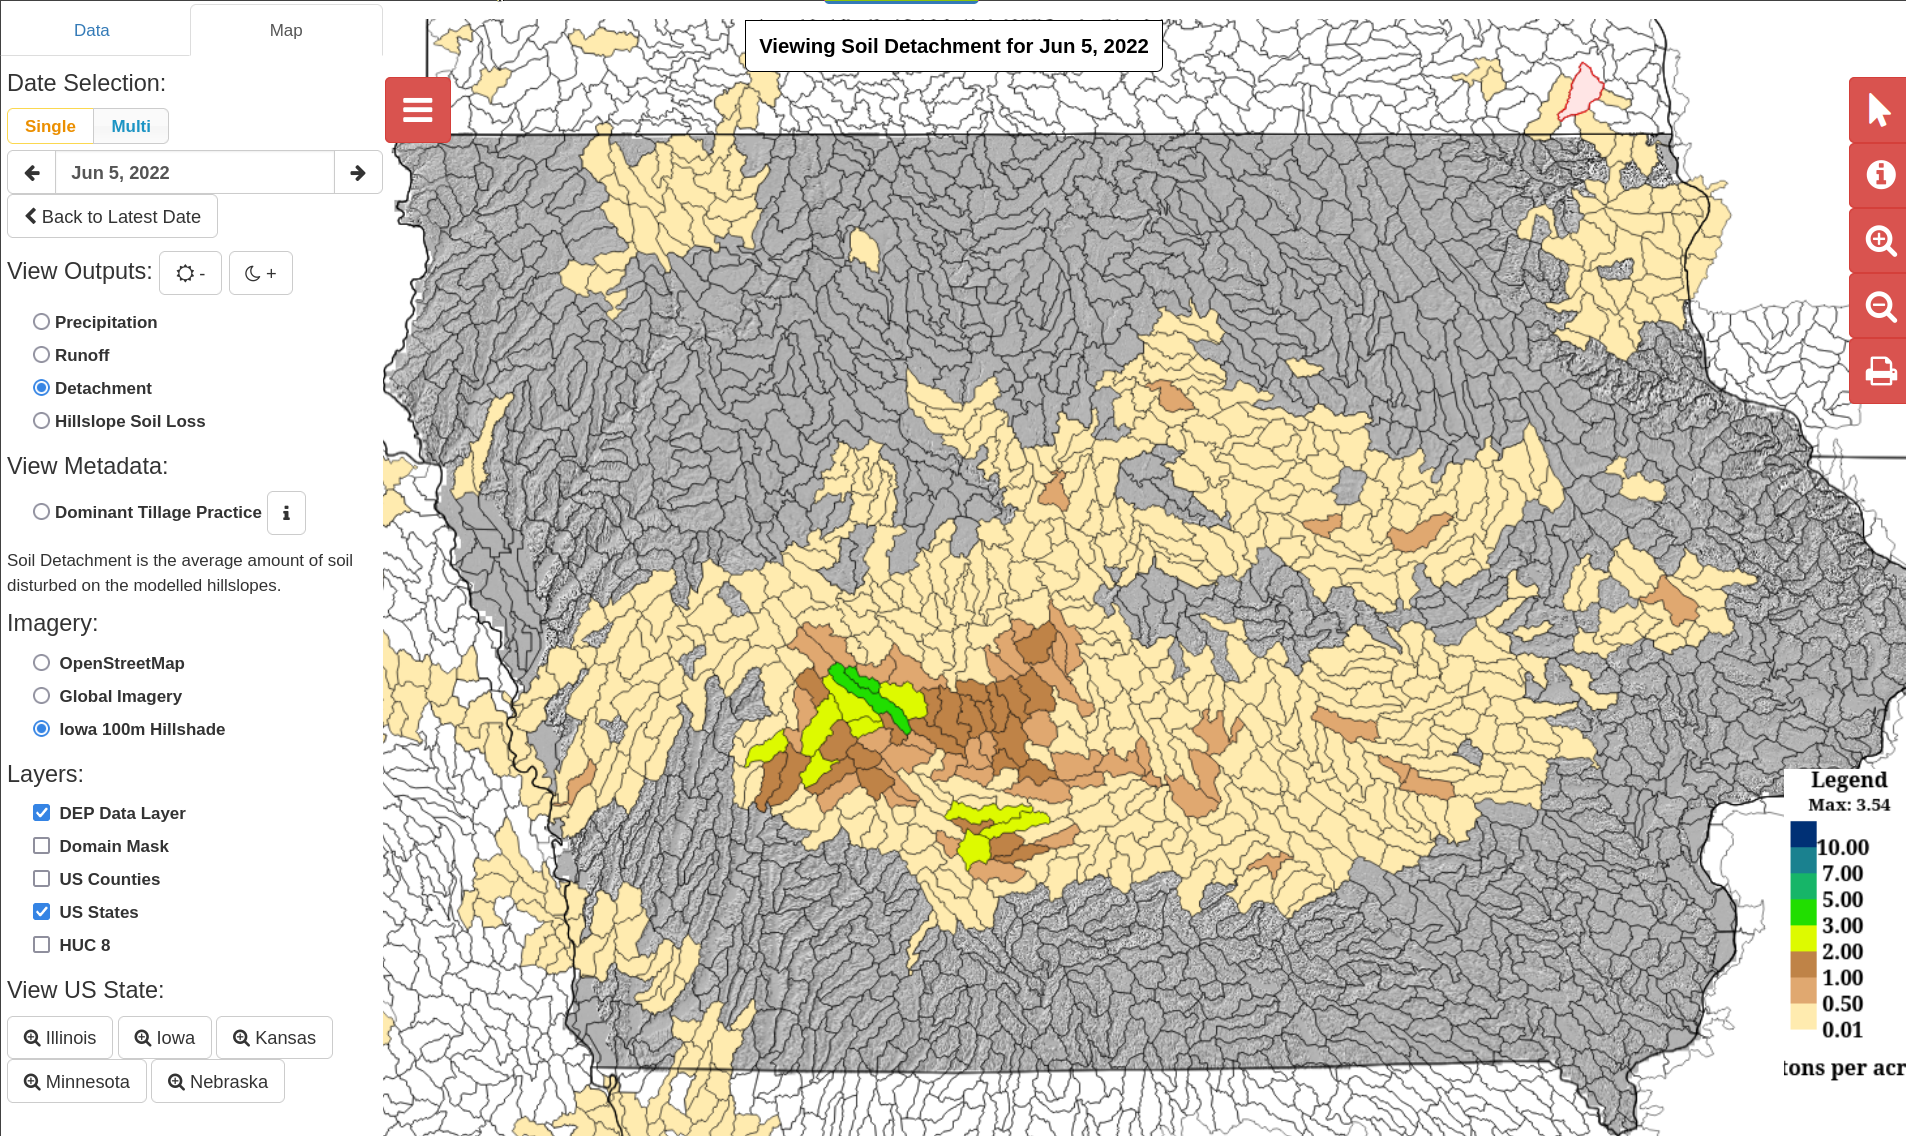
\includegraphics[width=.6\textwidth]{inc/dep_detachment_map_20220630_1610}
  \end{figure}

  {\tiny
    View interactive map here: 
  }

% https://www.dailyerosion.org/map/#20220601/20220630/avg_loss/-94.20/42.56/7.002790504174966//0/
  
  A 1-billion dollar loss
\end{frame}

\begin{frame}
  \frametitle{The science (2)}
  \framesubtitle{Explain the science here}

  \begin{figure}
    \centering
    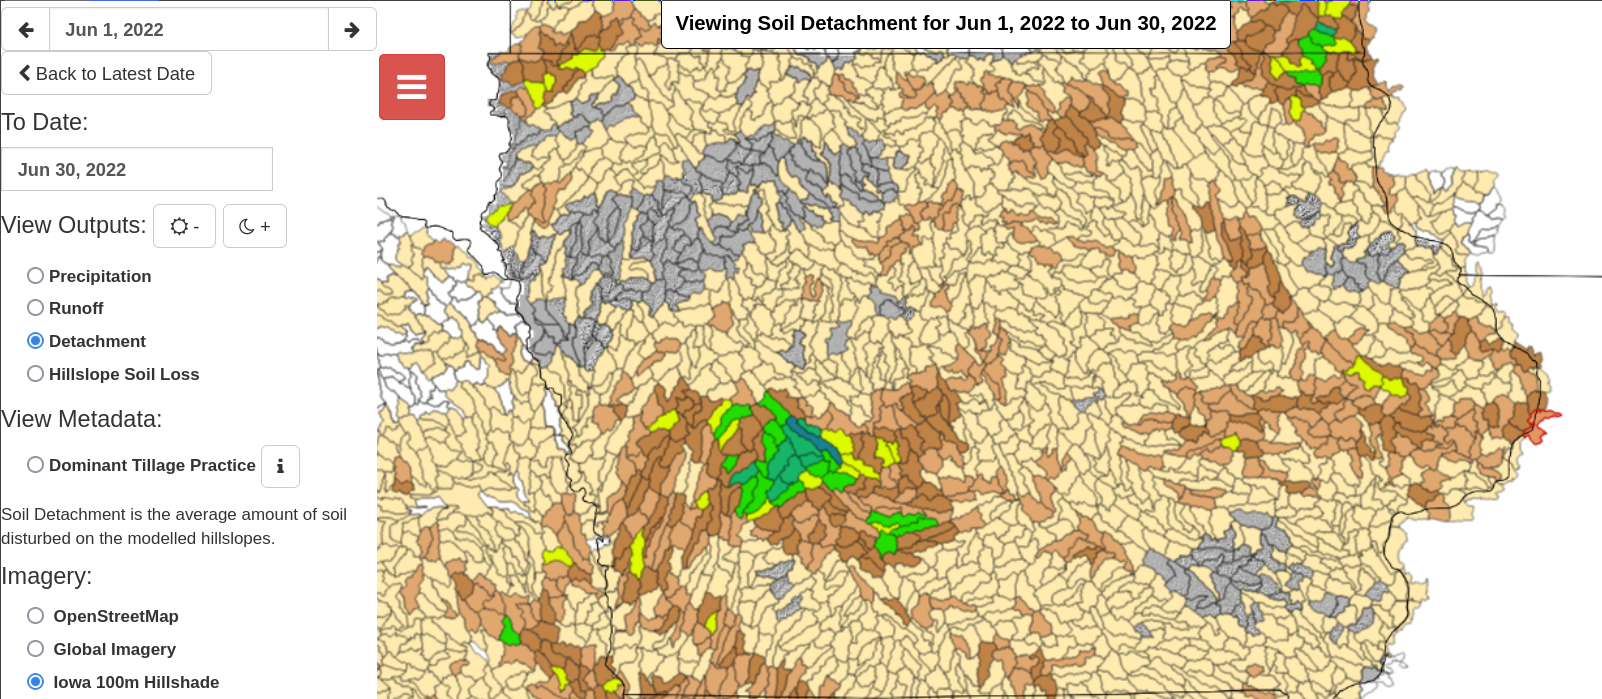
\includegraphics[width=.8\textwidth]{inc/dep_detachment_map_20220630_168}
  \end{figure}

  {\tiny
    View interactive map here: 
  }

% https://www.dailyerosion.org/map/#20220601/20220630/avg_loss/-94.20/42.56/7.002790504174966//0/
  A 1-billion dollar loss
\end{frame}


\begin{frame}
  \frametitle{Data}
  \framesubtitle{An example}

  Image with 3 or 4 facets and the Sel.Del as a number

  {\tiny
    Model documentation}
\end{frame}

\begin{frame}
  \frametitle{Methods}
  \framesubtitle{Model}

  Multiple vector, functional inputs

  Exact integral for piecewise linear models

  Math goes here
\end{frame}

\begin{frame}
  \frametitle{Methods}
  \framesubtitle{Implementation}

  Implementation (but skip it!)
\end{frame}

\begin{frame}
  \frametitle{Results}
  \framesubtitle{Posterior for model interpretation}

  Figure with posterior weights for fiGP, and also weights for vector inputs
\end{frame}

\begin{frame}
  \frametitle{Results}
  \framesubtitle{Prediction}

  Validation table
\end{frame}

% Discussion -------------------------------------------------------------------
\begin{frame}
  \frametitle{Discussion}
  \framesubtitle{My work}

  Toward a framework for Gaussian processes with functional inputs
  \begin{itemize}
  \item Framework for Gaussian processes with functional inputs
  \item Multiple vector and functional inputs
  \item Exact integral for piecewise linear inputs
  \item 3 functional weight forms
  \item 2 case studies
  \end{itemize}

  Future work
  \begin{itemize}
  \item In principle, should work with any inference / training paradigm
  \item Couple with local approximation for big datasets
  \end{itemize}
\end{frame}


% Closing slides ---------------------------------------------------------------
\begin{frame}[c]
  \frametitle{Acknowledgments}
  \centering

  {\small
    Benjamin Neo, Jarad Niemi, Max D. Morris (ISU) \\
    Margaret Johnson, Joaquim Texeira, Microwave Limb Sounder team
    (JPL, Caltech) \\
    Brian Gelder, Daryl Hermann, Rick Cruise (ISU) \\
    C-CHANGE:~Science for a Changing Agriculture \\
    Foundation for Food and Agriculture Research
  }

  \vfill

  {\huge Thank you!}

  \vfill

  {\tiny References and extra slides on the back}

  \href{ldamiano@iastate.edu}{\beamergotobutton{mail}
    ldamiano@iastate.edu}

  \href{https://github.com/luisdamiano/ANL22}{\beamergotobutton{repo}
https://github.com/luisdamiano/ANL22}
\end{frame}

\setbeamertemplate{bibliography item}{\insertbiblabel}
\begin{frame}[allowframebreaks]{References}
  \tiny
  \bibliographystyle{unsrt}
  \bibliography{references}
\end{frame}

% Appendix ---------------------------------------------------------------------
\section{Appendix}
\begin{frame}
  \frametitle{Trapezoidal approximation}

  \begin{figure}[h!]
    \centering
    \caption[]{Trapezoidal approximation}
  \end{figure}

  {
    \setlength{\abovedisplayskip}{-1cm}
    \begin{align}
      \int_{\mathcal{T}}
      \omega(t)
      {\left(X_i(t) - X_j(t) \right)}^2 dt
      \approx
      &
      \sum_{k = 2}^{K} {
      \left(t_{k} - t_{k - 1}\right)
      \frac{
      \Delta_{i, j, k} +
      \Delta_{i, j, k - 1}
      }{2}
      } \\
      \Delta_{i, j, k} =
      & \
      \omega(t_{k-1}) {\left(x_{i, k} - x_{j, k}\right)}^2
    \end{align}
  }

  \blankfootnote{See~\cite{muehlenstaedt2017} for a B-spline
    approach}
\end{frame}

\end{document}
